%! Author = Robert Kulesa, Daniel Liu, Michael Li
%! Date = 11/4/2021

% Preamble
\documentclass[11pt]{article}

% Packages
\usepackage{amsmath}
\usepackage{graphicx}

% Document
\begin{document}
    \begin{titlepage}
        \begin{center}
            \vspace{1cm}

            \Huge
            \textbf{Search Problems in AI}

            \vspace{0.5cm}
            \LARGE
            Assignment 2

            \vspace{1cm}

            \textbf{Michael Li - 192008938}

            \textbf{Daniel Liu - 184007283}

            \textbf{Robert Kulesa - 185009892}


            \vfill


            \vspace{0.8cm}

            \Large
            CS440 Fall 2021\\
            Professor Boularias\\
            Rutgers University - New Brunswick\\
            November 12, 2021

        \end{center}
    \end{titlepage}

    \begin{center}
        \Large
        \textbf{Problem 1}
    \end{center}
    \normalsize
    The sequence of nodes expanded by A* search, given the tree,
    and straight line distance heuristics, is in the following order:
    \begin{enumerate}
        \item[0.] $\left(city, f(city), g(city), h(city)\right)$
        \item $\left(\text{Lugoj}, 244, 0, 244\right)$
        \item $\left(\text{Mehadia}, 311, 70, 241\right)$
        \item $\left(\text{Lugoj}, 384, 140, 244\right)$
        \item $\left(\text{Drobeta}, 387, 145, 242\right)$
        \item $\left(\text{Craiova}, 425, 265, 160\right)$
        \item $\left(\text{Timisoara}, 440, 111, 329\right)$
        \item $\left(\text{Lugoj}, 446, 222, 244\right)$
        \item $\left(\text{Mehadia}, 451, 210, 241\right)$
        \item $\left(\text{Mehadia}, 461, 220, 241\right)$
        \item $\left(\text{Pitesti}, 503, 403, 100\right)$
        \item $\left(\text{Bucharest}, 504, 504, 0\right)$
    \end{enumerate}

    \begin{center}
        \Large
        \textbf{Problem 2}
    \end{center}
    \normalsize
    \begin{enumerate}
        \item[(a)] %insert explanation here
          BFS: $1 \rightarrow 2 \rightarrow 3\rightarrow 4 \rightarrow 5 \rightarrow 6 \rightarrow 7 \rightarrow 8 \rightarrow9\rightarrow10\rightarrow11$\\
          DLS: $1\rightarrow2\rightarrow4\rightarrow8\rightarrow9\rightarrow5\rightarrow10\rightarrow11$\\
          IDS: \\
          $1$\\
          $1\rightarrow2\rightarrow3$\\
          $1\rightarrow2\rightarrow3\rightarrow4\rightarrow5\rightarrow3\rightarrow6\rightarrow7$\\
          $1\rightarrow2\rightarrow4\rightarrow8\rightarrow9\rightarrow5\rightarrow10\rightarrow11$
        
        \item[(b)] %insert explanation here\\
        Bidirectional search would be effective in solving this problem.
        Bidirectionally finding a path between state 1 and state 11 reduces
        the number of nodes that needs to be explored.
        
        Forward   1\\
        Backward  11\\
        Forward   2\\
        Backward  5
        
        The branching factor is 2 in the forward direction and 1 in the reverse direction.
        
    \end{enumerate}

    \begin{center}
        \Large
        \textbf{Problem 3}
    \end{center}
    \normalsize
    \begin{enumerate}
        \item[(a)] True
        \item[(b)] True
        \item[(c)] True
        \item[(d)] False
        \item[(e)] False
        \item[(f)] True
        \item[(g)] True
        \item[(h)] True
        \item[(i)] True
    \end{enumerate}

    \begin{center}
        \Large
        \textbf{Problem 4}
    \end{center}
    \normalsize
    %insert explanation here

    \begin{center}
        \Large
        \textbf{Problem 5}
    \end{center}
    \normalsize
    %insert explanation here
    a)\\
    A heuristic is considered consistent iff:\\
        $h(n) \leq c(n,n+1) + h(n+1)$\\
        where h() is the heuristic and n is the goal state\\
        Proving by induction with the $n-1$ node in the shortest path to $n$ (base step):\\
        $h(n-1) \leq c(n-1,n) + h(n)$\\
        since n is the goal state, $h(n)=h^*(n)$, where $h^*(n)$ is the true minimal cost to the goal state\\
        $h(n) \leq c(n-1,n) + h^*(n)$\\
        given $c(n-1) + h^*(n) = h^*(n-1)$\\
        $h(n-1) \leq h^*(n-1)$\\
        which is the definition of admissibility\\\\
        Inductive Step with $n-2$:\\
        $h(n-2) \leq c(n-2,n-1) + h(n-1)$\\
        drawing from the base case:\\
        $h(n-2) \leq c(n-2,n-1) + h(n-1) \leq c(n-2,n-1) + h^*(n-1)$\\
        $h(n-2)\leq c(n-2,n-1) + h^*(n-1)$\\
        $h(n-2) \leq h^*(n-2)$\\
        By inductive reasoning, consistency implies admissibility\\\\
    b)\\
    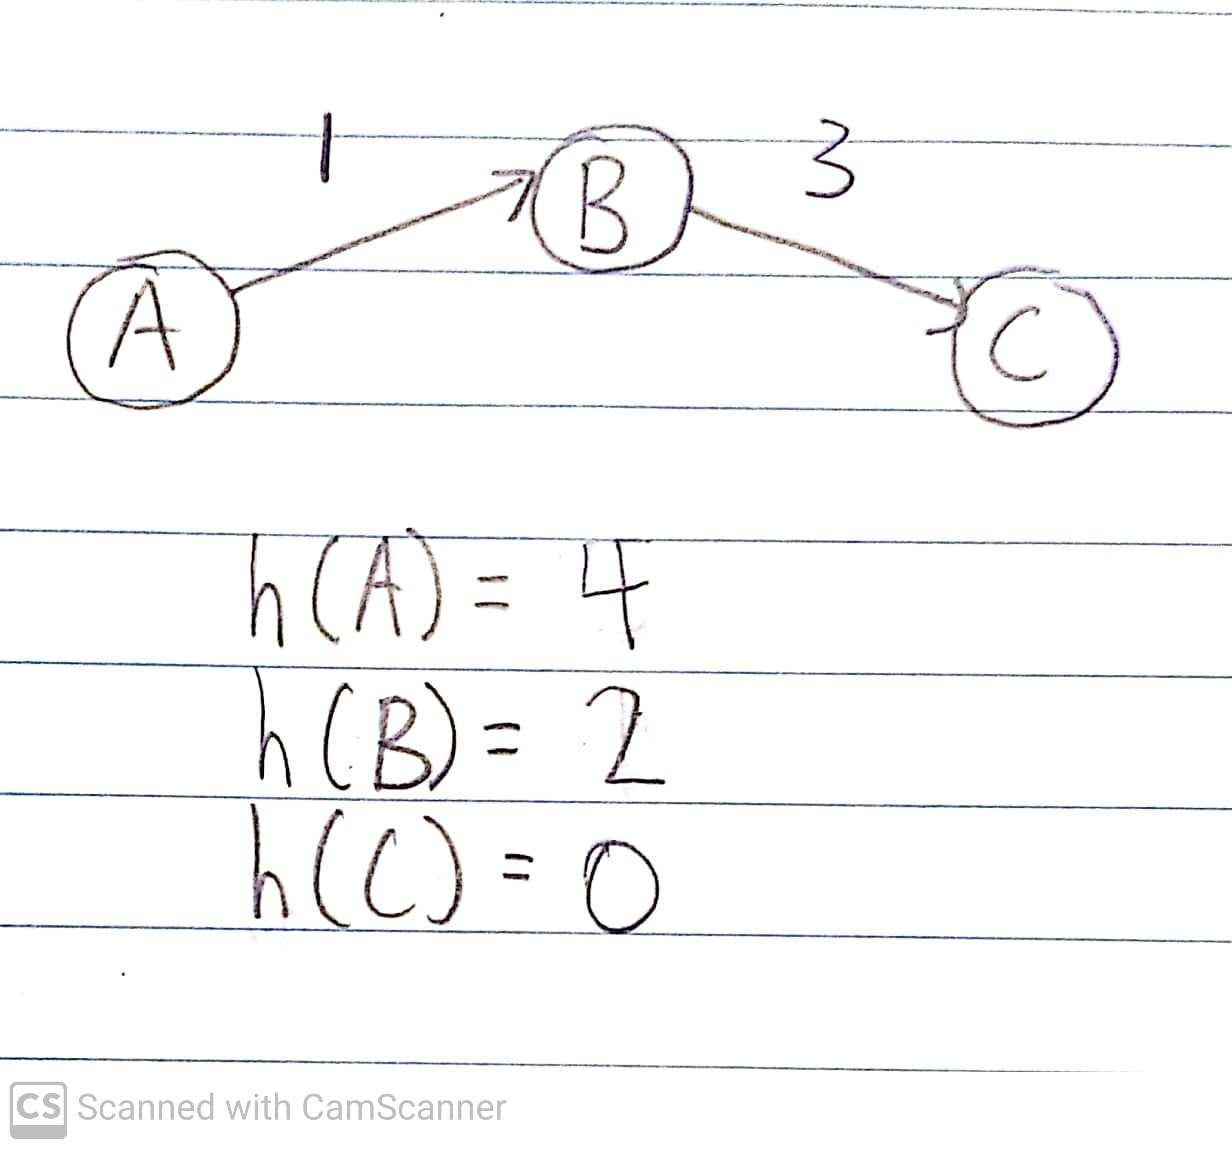
\includegraphics[width=0.9\textwidth]{images/prob_5_heuristic.jpg}
    
    \begin{center}
        \Large
        \textbf{Problem 6}
    \end{center}
    \normalsize
    In solving Constraint Satisfaction Problems, we choose the most constrained variable (MCV)
    in order to reduce the size of the next sub-problem.
    In other words, choosing the MCV maximally reduces the size of the next branch among
    any of the other variables. \\
    When assigning a value for this variable, we want to leave the remaining variables as unconstrained
    as possible in order to not accidentally eliminate any valid solutions.
    Thus, we want to assign the MCV the least constraining value (LCV).

    \begin{center}
        \Large
        \textbf{Problem 7}
    \end{center}
    \normalsize
    \begin{enumerate}
        \item[(a)]
            \begin{minipage}[!htb]{\linewidth}
                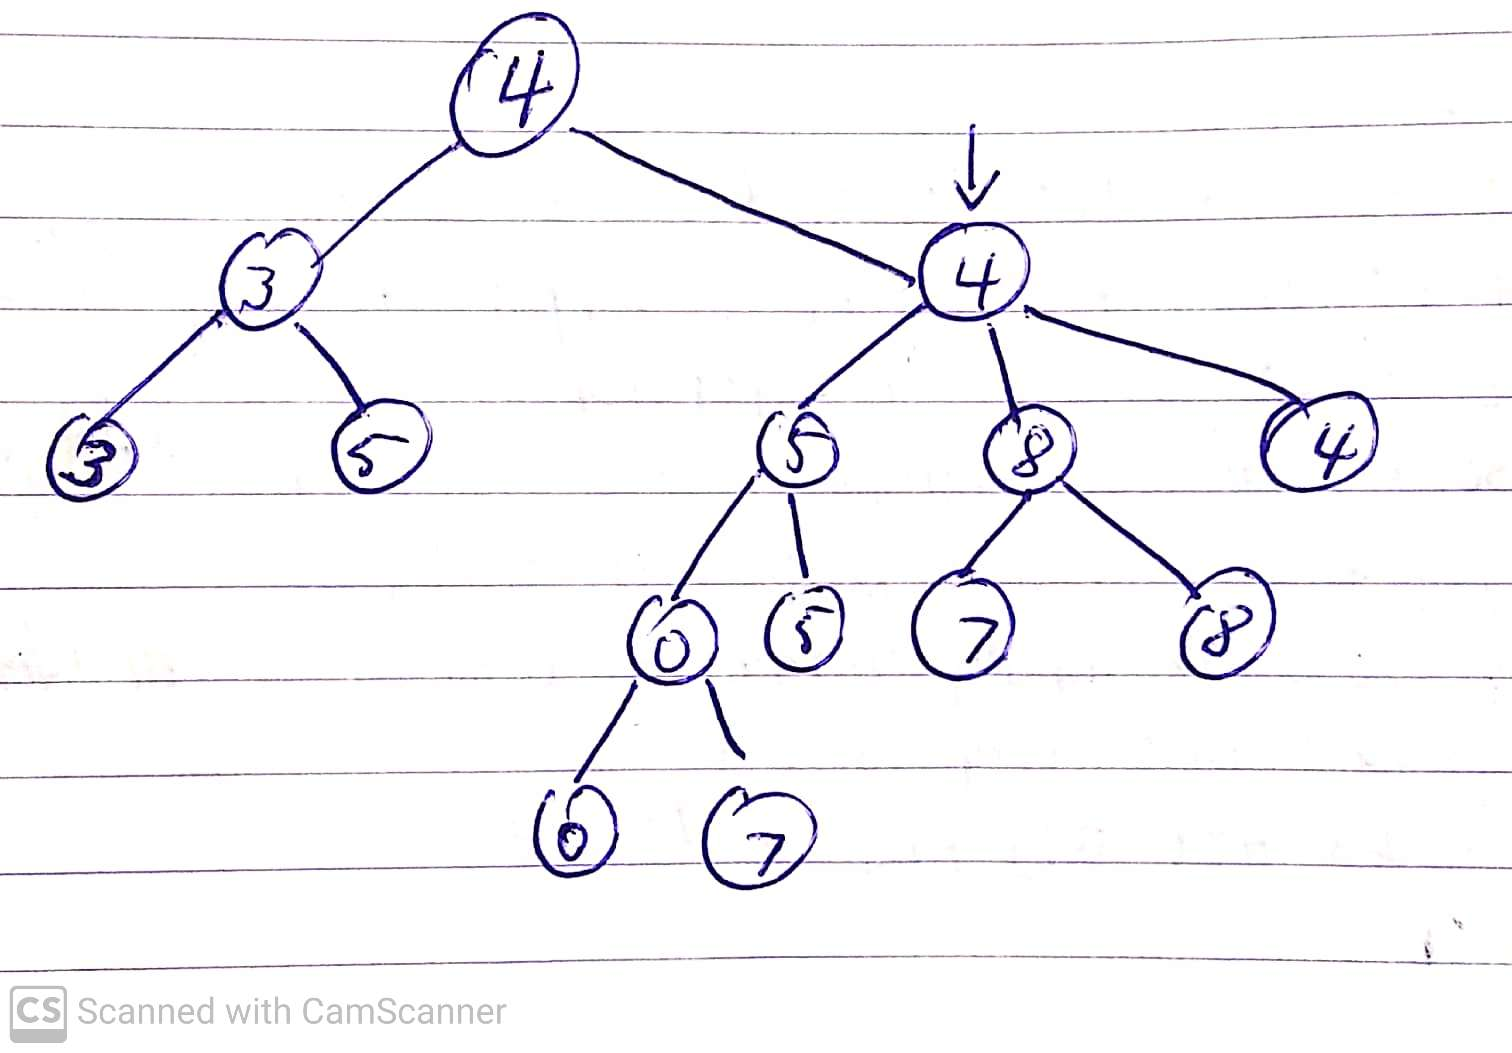
\includegraphics[width=\linewidth]{images/minmax_tree.jpg} \\
                \caption{The optimal choice for the max player would be the right node.}
            \end{minipage}

        \item[(b)] %insert explanation here
            \begin{minipage}[!htb]{\linewidth}
                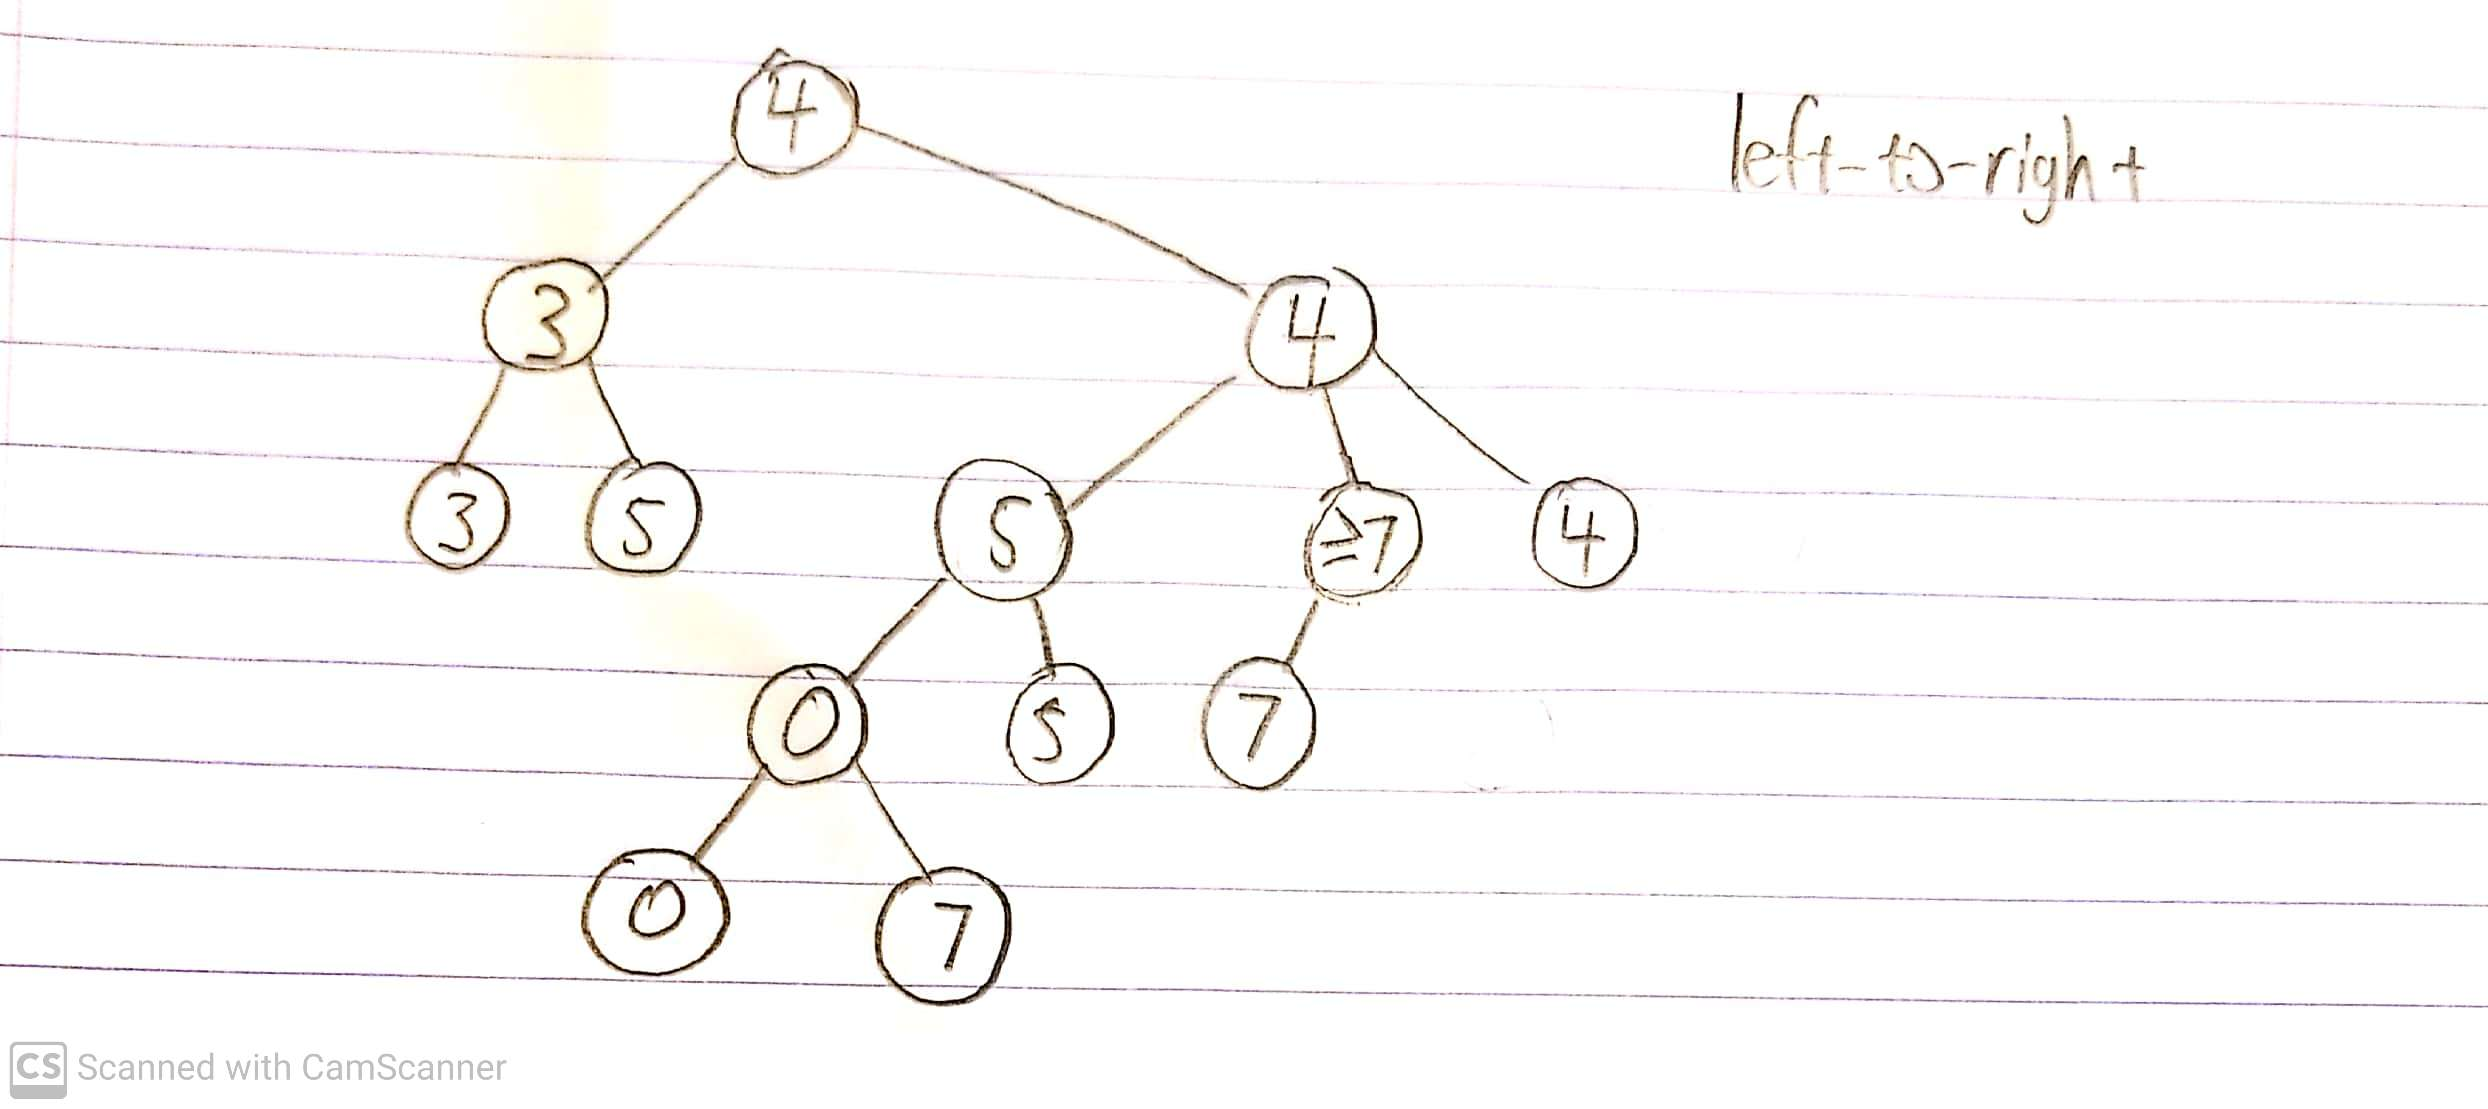
\includegraphics[width=\linewidth]{images/l2r_minmax_tree.jpg} \\
            \end{minipage}

        \item[(c)] %insert explanation here
            \begin{minipage}[!htb]{\linewidth}
                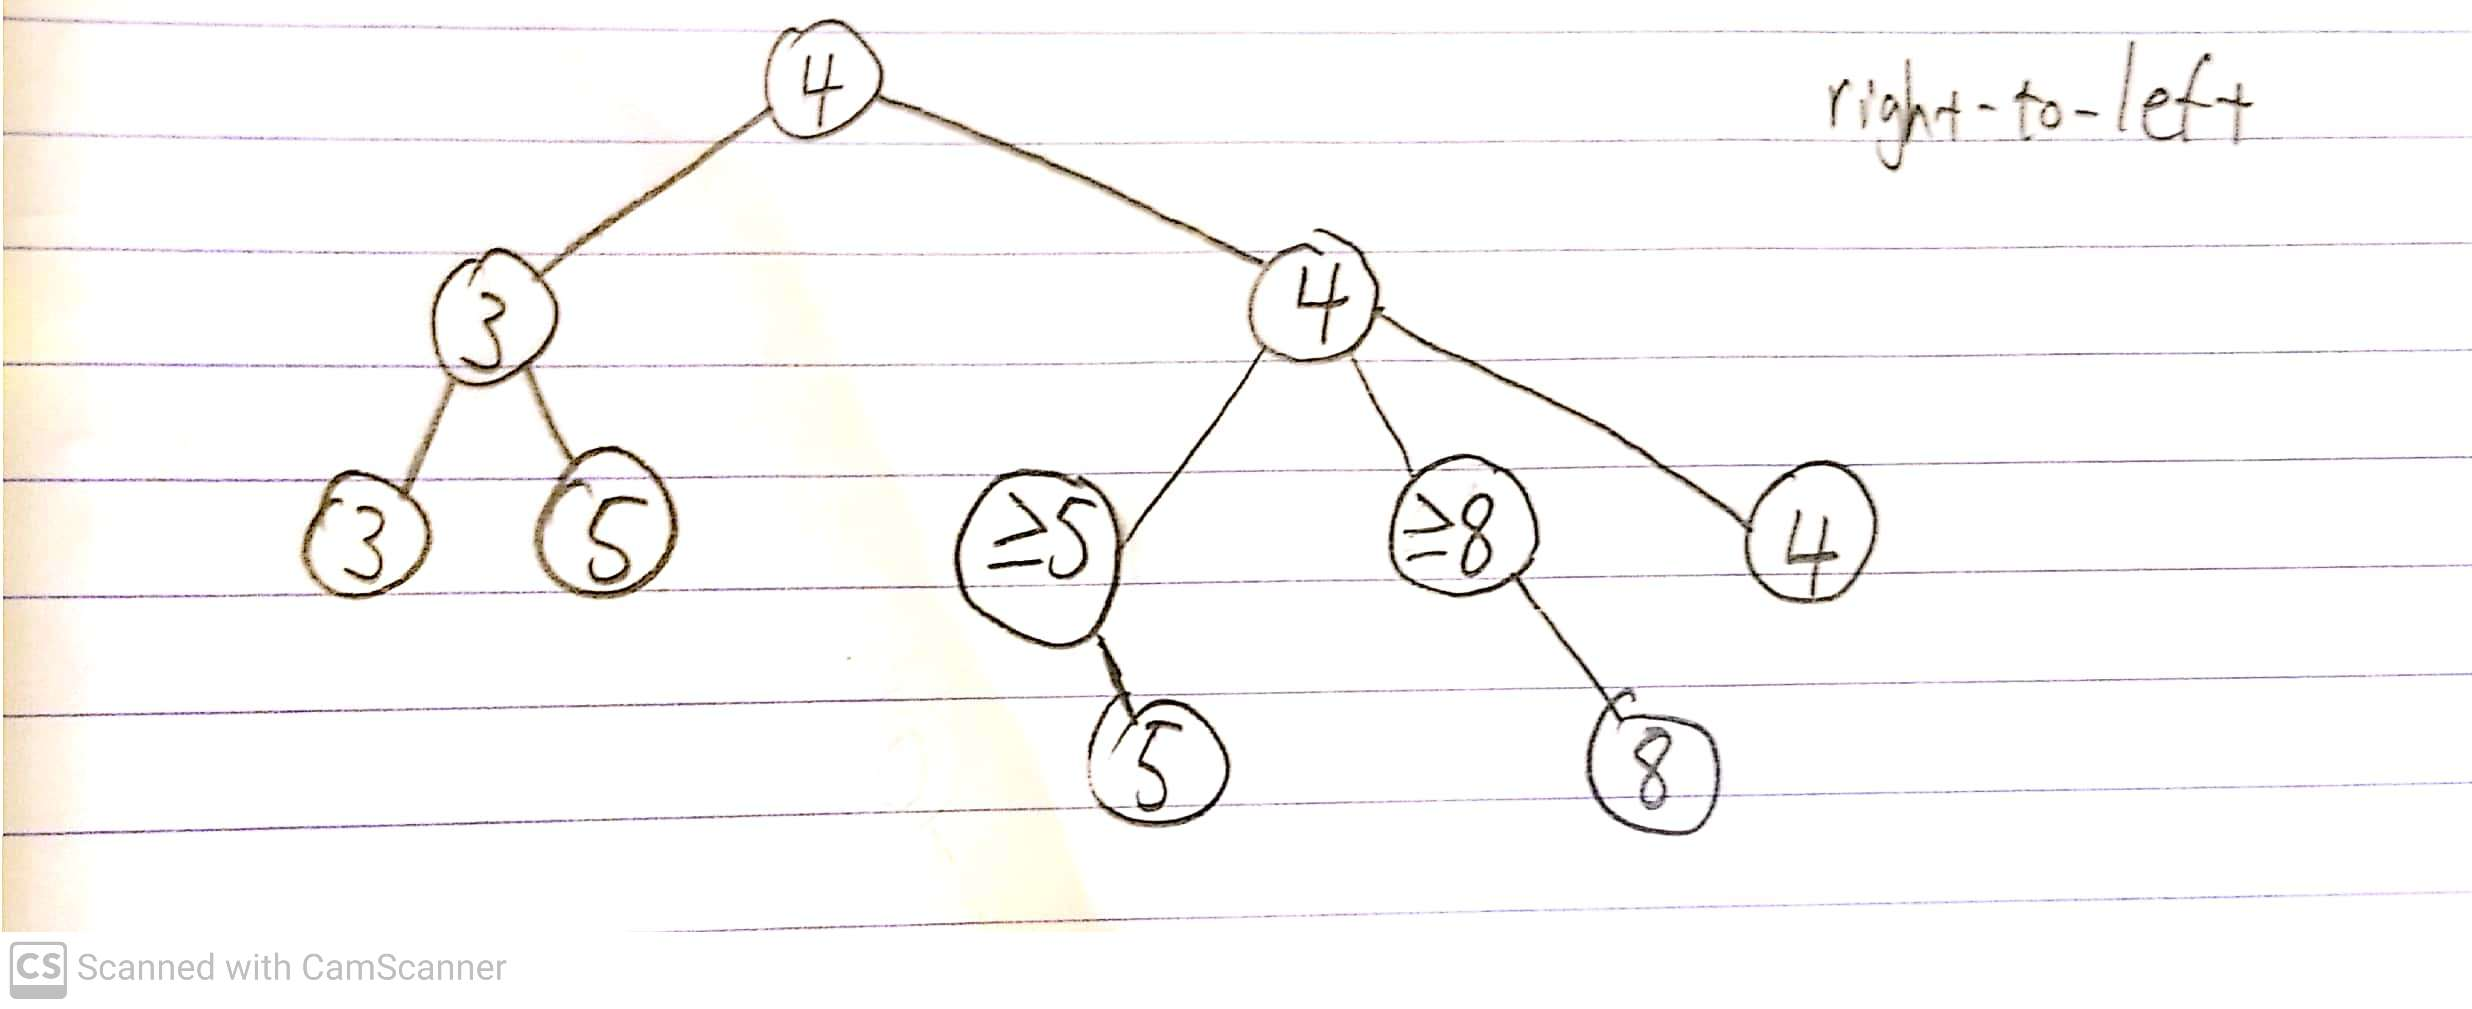
\includegraphics[width=\linewidth]{images/r2l_minmax_tree.jpg} \\
                Alpha-beta pruning is a heuristic that depends heavily on where elements are positioned, as it only operates on the best values found so far when exploring the tree. If the algorithm happens to find the 'best' node first then it can 'prune' more nodes from the tree. This is the case in right-to-left pruning, which, due to how the elements were positioned, was able to find the 'best' value more quickly and prune more nodes.
            \end{minipage}
    \end{enumerate}

    \begin{center}
        \Large
        \textbf{Problem 8}
    \end{center}
    \normalsize
    \begin{enumerate}
        \item[(a)] %insert explanation here
        \item[(b)] %insert explanation here
        \item[(c)] %insert explanation here
    \end{enumerate}

    \begin{center}
        \Large
        \textbf{Problem 9}
    \end{center}
    \normalsize
    \begin{enumerate}
        \item[(a)] %insert explanation here
        \item[(b)] %insert explanation here
        \item[(c)] %insert explanation here
        \item[(d)] %insert explanation here
        \item[(e)] %insert explanation here
        \item[(f)] %insert explanation here
    \end{enumerate}


\end{document}
